% NeuroAssist AI — Versão pt-BR
% Venue alvo: SBCAS 2027 (Simpósio Brasileiro de Computação Aplicada à Saúde)
% Template: SBC — baixar sbc-template.sty em https://www.sbc.org.br/documentos-da-sbc/summary/169-templates-para-artigos-e-capitulos-de-livros/878-modelosparapublicaodeartigos
% Compile: pdflatex main-ptbr.tex && bibtex main-ptbr && pdflatex main-ptbr.tex && pdflatex main-ptbr.tex
%
% ATENÇÃO — submissão SBCAS é CEGA (blind review):
%   Remover autoria, afiliação e agradecimentos pessoais antes de submeter.
%   Verificar se alguma referência interna identifica os autores.
%   Declarar uso de IA generativa no momento da submissão (conforme regra SBCAS 2026).

\documentclass[12pt]{article}

% ── Template SBC ──────────────────────────────────────────────────────────────
% O arquivo sbc-template.sty deve ser colocado neste diretório.
% Download: https://www.sbc.org.br/documentos-da-sbc/send/169-templates-para-artigos-e-capitulos-de-livros/878-modelosparapublicaodeartigos
\usepackage{sbc-template}

% Compatibilidade: sbc-template 2017 + LaTeX 2020+.
% \normalsfcodes é chamada no hook begindocument/before do babel mas não está
% inicializada. Registrar o fix no hook ANTES de carregar o babel garante FIFO.
\makeatletter
\AddToHook{begindocument/before}{%
  \def\normalsfcodes{\sfcode`\.\@m\sfcode`\?\@m\sfcode`\!\@m\sfcode`\:\@m\sfcode`\;\@m\sfcode`\,\@m}%
}
% Patch em \@outputpage para segurança nas páginas seguintes
\let\sbc@orig@outputpage\@outputpage
\def\@outputpage{%
  \def\normalsfcodes{\sfcode`\.\@m\sfcode`\?\@m\sfcode`\!\@m\sfcode`\:\@m\sfcode`\;\@m\sfcode`\,\@m}%
  \sbc@orig@outputpage}
\makeatother

% ── Pacotes ───────────────────────────────────────────────────────────────────
\usepackage[brazilian]{babel}
\usepackage[utf8]{inputenc}
\usepackage[T1]{fontenc}
\usepackage{graphicx}
\usepackage{booktabs}
\usepackage{amsmath,amssymb}
\usepackage{url}
\usepackage{hyperref}
\usepackage{listings}
\usepackage{xcolor}
\usepackage{tikz}

\lstset{basicstyle=\ttfamily\footnotesize, breaklines=true}

% Placeholder de rascunho — remover antes da submissão
\newcommand{\fillme}[1]{\textcolor{red}{\textsf{[#1]}}}

% ── Título e autores ──────────────────────────────────────────────────────────
% REMOVER autoria para submissão cega
\title{NeuroAssist AI: Uma Plataforma Offline-First e Preservadora de Privacidade
para Comunicação Assistiva Baseada em Gestos Faciais Residuais
em Doenças Neurodegenerativas}

\author{Danilo Amaral\inst{1}}

\address{TechLab AI\\
  cybernautta@gmail.com}

% Chamar \normalsize para inicializar \normalsfcodes antes do hook begindocument/before do babel
\normalsize

\begin{document}

\maketitle

% ── Resumo ────────────────────────────────────────────────────────────────────
\begin{resumo}
Pacientes com doença do neurônio motor (DNM/ELA) perdem progressivamente o controle
motor voluntário, frequentemente retendo apenas movimentos faciais sutis como último
canal de comunicação. Os sistemas de comunicação aumentativa e alternativa (CAA)
existentes requerem conectividade de rede estável e não se adaptam ao perfil motor
residual individual do paciente. Apresentamos o NeuroAssist AI, uma plataforma de
comunicação assistiva offline-first e preservadora de privacidade que transforma
gestos faciais residuais em solicitações de emergência estruturadas, utilizando um
pipeline de visão computacional baseado em WebAssembly executado localmente. O
sistema combina uma máquina de estados de seis estados para reconhecimento de gesto
deliberado com calibração de limiar EAR específica por paciente, implantado sobre
uma arquitetura de microsserviços hexagonal. Avaliamos o sistema com um paciente
DNM em estágio avançado e cinco cuidadores e voluntários em um estudo de caso
preliminar. A latência ponta-a-ponta da conclusão do gesto até a exibição do alarme
ao cuidador foi em média \textbf{[X]}\,ms ($\sigma$\,=\,[Y]\,ms) em [N] tentativas.
A máquina de estados de gesto deliberado reduziu a taxa de falsos positivos de
[A]\,\% (limiar EAR simples) para [B]\,\% ([N] participantes). O NeuroAssist AI
demonstra que a detecção precisa e preservadora de privacidade de gestos residuais
é alcançável em hardware comum sem dependência de rede, usando uma arquitetura
calibrável e extensível validada em contexto real de cuidado domiciliar de DNM.
\end{resumo}

% ── Abstract (inglês) ─────────────────────────────────────────────────────────
\begin{abstract}
Patients with motor neurone disease (MND/ALS) progressively lose voluntary motor
control, often retaining only subtle facial movements as their last communication
channel. Existing augmentative and alternative communication (AAC) systems require
reliable network connectivity and do not adapt to the residual motor profile of
individual patients. We present NeuroAssist AI, a privacy-preserving, offline-first
assistive communication platform that transforms residual facial gestures into
structured emergency requests using a locally executed WebAssembly-based computer
vision pipeline. The system combines a six-state deliberate gesture recognition
state machine with patient-specific EAR threshold calibration, deployed over a
hexagonal microservices architecture. End-to-end latency averaged [X]\,ms
($\sigma$\,=\,[Y]) across [N] trials. The state machine reduced the false-positive
rate from [A]\,\% to [B]\,\%. NeuroAssist AI demonstrates that high-accuracy,
privacy-preserving residual gesture detection is achievable on commodity hardware
without network dependency.
\end{abstract}

% ── Seções ────────────────────────────────────────────────────────────────────
% =============================================================================
% Seção 1 — Introdução
% =============================================================================

\section{Introdução}
\label{sec:introducao}

A esclerose lateral amiotrófica (ELA), internacionalmente denominada motor neurone disease
(MND) ou amyotrophic lateral sclerosis (ALS), é uma condição neurodegenerativa progressiva que destrói os neurônios motores
superiores e inferiores, resultando em perda de movimento voluntário, fala e, por fim,
função respiratória. A incidência global é de aproximadamente 2--3 casos por
100.000 pessoas-ano, afetando cerca de 41.000 indivíduos na Austrália e 30.000 no
Brasil~\cite{mehta2018mnd}. A sobrevida mediana após o diagnóstico é de 2--5 anos; a
insuficiência respiratória, tipicamente tratada com ventilação não invasiva (VNI), é
a principal causa de morte. Notavelmente, a VNI demonstrou prolongar a sobrevida por
um fator de aproximadamente três em comparação ao melhor tratamento farmacológico
disponível~\cite{berlowitz2021niv}, tornando o período de uso da VNI clinicamente
significativo e prolongado. Durante essa fase, os pacientes permanecem cognitivamente
intactos enquanto se tornam progressivamente incapazes de falar ou gesticular de
formas que as tecnologias de comunicação padrão consigam detectar.

Trabalhos recentes demonstraram que a assincronia paciente-ventilador (PVA) — uma
incompatibilidade entre os ciclos do ventilador e o esforço respiratório do paciente
— é um contribuinte significativo para a não adesão à VNI na ELA, causando
desconforto, fragmentação do sono e potencialmente desfechos clínicos
adversos~\cite{atkeson2011pva, yang2026pva, berlowitz2025tla}. Pacientes que
experimentam desconforto relacionado à PVA durante o uso noturno da VNI não
conseguem sinalizar angústia facilmente aos cuidadores usando as tecnologias de CAA
existentes, que requerem conectividade de rede ou hardware dedicado inadequado para
o ambiente domiciliar. O NeuroAssist AI aborda diretamente essa lacuna: ao fornecer
um canal de sinalização local e sempre disponível que requer apenas uma webcam comum,
permite que os pacientes alertem os cuidadores durante períodos sem supervisão —
incluindo enquanto utilizam a VNI à noite.

Em estágios avançados, uma proporção substancial de pacientes experimenta uma condição
semelhante ao locked-in, na qual o controle voluntário se limita a movimentos faciais
residuais sutis: pequenas contrações palpebrais, elevações de sobrancelha ou
microexpressões que persistem após a perda da função motora dos membros e orofacial.
Esses gestos residuais representam o último canal voluntário disponível para
comunicação. Sem um meio confiável de detectá-los e agir sobre eles, os pacientes não
conseguem sinalizar angústia, desconforto ou necessidades aos cuidadores — com
consequências diretas para a qualidade de vida e a segurança do paciente durante
períodos sem assistência.

Os sistemas de comunicação aumentativa e alternativa (CAA) existentes não atendem
adequadamente essa população. Dispositivos de rastreamento ocular de ponta (e.g.,
Tobii Dynavox) e softwares de CAA dedicados (e.g., Grid~3) oferecem alta precisão,
mas requerem conectividade sem fio estável, hardware dedicado custando mais de
USD~3.000, e configurações calibradas em fábrica que não conseguem se adaptar ao
perfil motor em declínio de um paciente individual~\cite{beukelman2013aac}.
Interfaces cérebro-computador (BCI) via EEG oferecem uma alternativa, mas envolvem
hardware invasivo ou volumoso inadequado para implantação domiciliar~\cite{zander2011passive}.
Abordagens baseadas em câmera de baixo custo existem na literatura~\cite{soukupova2016},
mas dependem de comparações simples de limiar por quadro que geram taxas de falsos
positivos inaceitavelmente altas quando aplicadas à atividade facial involuntária
presente em pacientes com ELA durante a VNI.

Apresentamos o \textbf{NeuroAssist AI}, uma plataforma de comunicação assistiva
offline-first e preservadora de privacidade projetada para implantação domiciliar com
uma webcam comum. O sistema transforma gestos faciais residuais em solicitações de
emergência estruturadas usando um pipeline de visão computacional WebAssembly
executado localmente, uma máquina de estados de gesto deliberado e um perfil de
detecção calibrável por paciente — sem transmitir nenhum vídeo para fora do
dispositivo.

Este artigo apresenta três contribuições originais:
\begin{enumerate}
  \item \textbf{Um pipeline de detecção offline-first e preservador de privacidade.}
    O modelo MediaPipe FaceLandmarker e seu runtime WebAssembly são servidos a partir
    de ativos locais; nenhum quadro de vídeo ou dado biométrico sai do dispositivo
    do paciente. O delegate de CPU garante compatibilidade com hardware comum,
    independentemente da disponibilidade de GPU.

  \item \textbf{Uma máquina de estados de gesto deliberado de seis estados com
    calibração específica por paciente.}
    Em vez de um único limiar EAR, a máquina de estados exige duração mínima de
    fechamento ($\geq$3 quadros, ${\approx}$100\,ms) em cada uma de duas piscadas
    sequenciais, reabertura confirmada entre elas, e uma janela de tempo configurável.
    Os limiares são armazenados em um \texttt{DetectionProfile} versionado e adaptados
    por paciente. Esse design aborda especificamente as fontes de falsos positivos
    relevantes para a ELA: piscadas involuntárias, artefatos de ptose parcial e
    deriva lenta de limiar.

  \item \textbf{Uma arquitetura extensível de microsserviços hexagonais com tipos de
    gesto plug-in.}
    O campo \texttt{engineFeatureRef} no perfil de detecção desacopla o motor de
    reconhecimento de gesto do catálogo de comandos, permitindo que novos gestos
    (elevação de sobrancelha, piscada de um olho) sejam registrados sem modificar o
    código de domínio existente. Regras ArchUnit aplicadas em tempo de compilação
    garantem que essa separação persista à medida que o sistema evolui.
\end{enumerate}

O restante do artigo está organizado da seguinte forma. A Seção~\ref{sec:relacionados}
revisa os trabalhos relacionados em CAA, detecção de gesto facial e computação de
borda para saúde. A Seção~\ref{sec:arquitetura} descreve a arquitetura do sistema em
detalhe. A Seção~\ref{sec:avaliacao} relata a avaliação experimental. A
Seção~\ref{sec:discussao} discute limitações e trabalhos futuros, e a
Seção~\ref{sec:conclusao} conclui o artigo.

% =============================================================================
% Seção 2 — Trabalhos Relacionados
% =============================================================================

\section{Trabalhos Relacionados}
\label{sec:relacionados}

\subsection{Sistemas de CAA para Doenças Neurodegenerativas}

A comunicação aumentativa e alternativa (CAA) para pessoas com ELA tem sido
estudada extensivamente desde a década de 1990~\cite{beukelman2013aac}. Soluções
comerciais dominam a prática clínica: dispositivos de rastreamento ocular de ponta,
como o Tobii Dynavox PCEye e o Eyegaze Edge, oferecem seleção por olhar com precisão
superior a 98\,\% em condições laboratoriais, mas apresentam custos de hardware acima
de USD~3.000 e requerem recalibração periódica por profissionais treinados~\cite{beukelman2013aac}.
Esses sistemas pressupõem controle oculomotor residual suficiente, que se deteriora
à medida que a ELA progride em direção à oftalmoplegia. Pacotes de software de CAA
como o Grid~3 dependem de conectividade Bluetooth ou Wi-Fi estável para sincronizar
conjuntos de símbolos e perfis de usuário, criando uma barreira para usuários
domiciliares sem banda larga confiável.

Uma pesquisa de Clarke et al.~\cite{clarke2021aac} identificou que a provisão de CAA
para pessoas com ELA é caracterizada por encaminhamento tardio, transições rápidas de
dispositivos à medida que a função motora declina, e uma lacuna persistente em soluções
de baixo custo e adaptáveis adequadas para o ambiente domiciliar. As interfaces
cérebro-computador (BCI) via eletroencefalografia oferecem um caminho alternativo que
contorna o sistema motor por completo, mas os headsets de BCI não invasivos atuais
atingem taxas típicas de transferência de informação de 5--25 bits por minuto em
condições ótimas, requerem operadores treinados e são inadequados para o contexto de
cuidado domiciliar~\cite{zander2011passive}. BCIs corticais implantadas atingem taxas
maiores, mas apresentam risco cirúrgico. O NeuroAssist AI visa o estágio intermediário
— após a perda da função dos membros e da fala, mas enquanto persiste algum grau de
movimento facial voluntário — para o qual não existe atualmente nenhuma solução de
baixo custo e independente de rede na literatura.

\subsection{Detecção de Gesto Facial via Visão Computacional}

Três gerações de análise facial baseada em câmera são relevantes para este trabalho.

\emph{Primeira geração — classificadores em cascata.} Viola e Jones~\cite{violajones2004}
introduziram a detecção de faces em tempo real usando cascatas de características Haar,
permitindo a implantação em hardware de consumo. Esses detectores localizam o rosto,
mas não fornecem coordenadas de marcos sub-faciais; a detecção de piscadas requer
heurísticas adicionais aplicadas à região do olho detectada e é altamente sensível a
variações de iluminação.

\emph{Segunda geração — regressão de marcos faciais.} A biblioteca Dlib de King~\cite{king2009dlib}
popularizou a detecção de 68 marcos faciais por meio de um conjunto de árvores de
regressão, permitindo o cálculo confiável do EAR~\cite{soukupova2016} sem aprendizado
profundo. Soukupová e Čech~\cite{soukupova2016} formalizaram o EAR como um escalar
único para detecção de piscadas, demonstrando precisão de detecção em nível de quadro
acima de 99\,\% em conjuntos de dados controlados. A principal limitação dessa geração
é a ausência de um runtime compatível com WebAssembly, tornando a implantação no
navegador do lado do cliente impraticável.

\emph{Terceira geração — modelos de marcos profundos no dispositivo.} O MediaPipe
FaceLandmarker~\cite{lugaresi2019mediapipe} fornece 468 marcos faciais normalizados e
52 coeficientes de blendshape a aproximadamente 30\,fps em um contexto de navegador
WebAssembly usando apenas um delegate de CPU. O NeuroAssist AI se baseia nessa
geração, retendo o EAR para a máquina de estados de dupla piscada (onde sua
simplicidade auxilia a interpretabilidade) enquanto usa pontuações de blendshape para
gestos de piscada de um olho e sobrancelha.

\subsection{Reconhecimento de Gesto Deliberado e Supressão de Falsos Positivos}

Um desafio fundamental em CAA acionada por gesto é distinguir ativações intencionais
da atividade facial involuntária que ocorre continuamente durante o comportamento normal.
A taxa de piscadas espontâneas em adultos saudáveis é de 15--20 piscadas por
minuto~\cite{bentivoglio1997}; em pacientes com ELA, as taxas podem ser menores devido
à perda de neurônios motores, mas permanecem diferentes de zero. Qualquer abordagem
baseada em limiar aplicada no nível de quadro único produz taxas de falsos positivos
da ordem de vários por minuto em condições naturais, tornando o monitoramento sem
supervisão inviável.

As duas principais estratégias na literatura para suprimir falsos positivos em CAA
facial são \emph{tempo de permanência} (\emph{dwell time}) e \emph{modelagem de
intencionalidade}. A seleção por tempo de permanência — amplamente usada em CAA
baseada em olhar — exige que o usuário fixe uma região-alvo por uma duração fixa
(tipicamente 0,5--1\,s)~\cite{majaranta2002eyetyping}. Essa abordagem é inaplicável
à entrada baseada em piscada, pois uma piscada por definição fecha o olho e interrompe
a fixação. A modelagem de intencionalidade via máquinas de estados foi proposta na
literatura mais ampla de interação humano-computador~\cite{zander2011passive}, mas sua
aplicação à CAA baseada em piscada para ELA não foi sistematicamente descrita. A
máquina de seis estados introduzida neste artigo (Seção~\ref{sec:maquinadeestados})
aplica restrições de intencionalidade específicas ao gesto de dupla piscada: duração
mínima de fechamento por piscada, abertura confirmada entre piscadas, e uma janela
temporal — combinação não encontrada, ao conhecimento dos autores, na literatura
anterior de CAA.

\subsection{Computação de Borda e Privacidade para Aplicações de Saúde}

O processamento de dados de sensores relacionados à saúde no dispositivo, em vez de
na nuvem, tem recebido atenção crescente após a aplicação do GDPR em 2018 e da LGPD
em 2020~\cite{edpb2020privacy}. O vídeo facial é classificado explicitamente como dado
biométrico sob ambos os marcos regulatórios, atraindo as maiores obrigações regulatórias
de processamento. A execução local via WebAssembly fornece uma garantia prática de
privacidade: o modelo de execução com memória isolada da especificação impede que um
módulo carregado acesse qualquer estado do navegador fora de sua memória linear, e
nenhuma chamada de rede é necessária para executar a inferência do marcador de
landmark~\cite{haas2017wasm}. A latência de implantação de modelos WebAssembly para
análise facial foi relatada em 20--40\,ms por quadro em hardware de consumo sem
aceleração por GPU~\cite{lugaresi2019mediapipe}, consistente com a operação a 30\,fps
observada em nosso PoC.

\subsection{Arquitetura de Software para Sistemas de Saúde}

A arquitetura Hexagonal (Portas e Adaptadores)~\cite{cockburn2005hexagonal} foi
proposta como um padrão estrutural para sistemas de informação em saúde onde o modelo
de domínio deve permanecer isolado de mudanças tecnológicas — um requisito recorrente
em software de saúde regulamentado onde requisitos de auditoria, esquemas de dados e
padrões de integração evoluem de forma independente~\cite{richardson2018microservices}.
A decomposição em microsserviços de plataformas de CAA não foi relatada na literatura,
ao conhecimento dos autores; a maioria dos sistemas existentes são aplicações
monolíticas de desktop ou firmware. A arquitetura do NeuroAssist AI demonstra que
decompor um pipeline de gesto-para-alarme em serviços independentemente implantáveis
é viável em escala de PoC, e que a aplicação de limites em tempo de compilação via
ArchUnit fornece um mecanismo prático para manter a disciplina hexagonal.

\subsection{Comunicação e Segurança Durante o Uso de VNI na ELA}

A adesão à ventilação não invasiva na ELA está consistentemente abaixo das metas
clínicas, com desconforto relatado pelo paciente e assincronia dispositivo-paciente
identificados como principais fatores contribuintes~\cite{berlowitz2021niv, yang2026pva}.
A polissonografia domiciliar em 23 pacientes com ELA utilizando VNI noturna documentou
um índice de assincronia médio de 69 eventos por hora (intervalo 15--146) — muito
acima dos limiares associados à perturbação clinicamente significativa do
sono~\cite{atkeson2011pva}. O ensaio clínico randomizado 3TLA~\cite{berlowitz2025tla}
investiga atualmente se a titulação da VNI guiada por polissonografia melhora as taxas
de uso; seu desfecho primário — uso de VNI superior a quatro horas por dia — reflete
o desafio de manter a adesão em ambientes domiciliares. Uma dimensão complementar e
pouco explorada é a capacidade do paciente de sinalizar desconforto ou angústia aos
cuidadores durante o uso de VNI sem supervisão, particularmente à noite. Ao conhecimento
dos autores, nenhum sistema publicado fornece um mecanismo independente de rede e de
baixo custo para esse fim; o NeuroAssist AI foi projetado para preencher essa lacuna.

% =============================================================================
% Seção 3 — Arquitetura do Sistema
% =============================================================================

\section{Arquitetura do Sistema}
\label{sec:arquitetura}

O NeuroAssist AI é composto por dois contextos implantáveis: um \emph{pipeline de
detecção no navegador}, executado inteiramente no dispositivo do paciente, e um
\emph{pipeline de alertas no backend}, implementado como microsserviços hexagonais.
A Figura~\ref{fig:visaogeral} ilustra o fluxo de dados ponta-a-ponta.

\subsection{Visão Geral do Sistema}
\label{sec:visaogeral}

O pipeline é acionado por um gesto facial deliberado capturado por qualquer webcam
comum (720\,p ou superior). O loop de detecção de gestos é executado exclusivamente
no navegador via WebAssembly; nenhum quadro de vídeo sai do dispositivo em nenhum
momento. Quando um gesto é confirmado pela máquina de estados
(Seção~\ref{sec:maquinadeestados}), um payload JSON leve é enviado via POST ao serviço
de ingestão de eventos. O serviço valida o gesto contra o perfil de detecção ativo do
paciente, cria um registro \texttt{Evento} e despacha uma notificação
\texttt{FULL\_SCREEN\_ALARM}. A aplicação do cuidador consulta o backend a cada cinco
segundos; ao detectar um evento ativo, renderiza uma sobreposição de alarme em tela
cheia. O cuidador confirma o atendimento, o que grava um \texttt{verdict} de volta ao
registro do evento e limpa o alarme.

\begin{figure*}[!t]
  \centering
  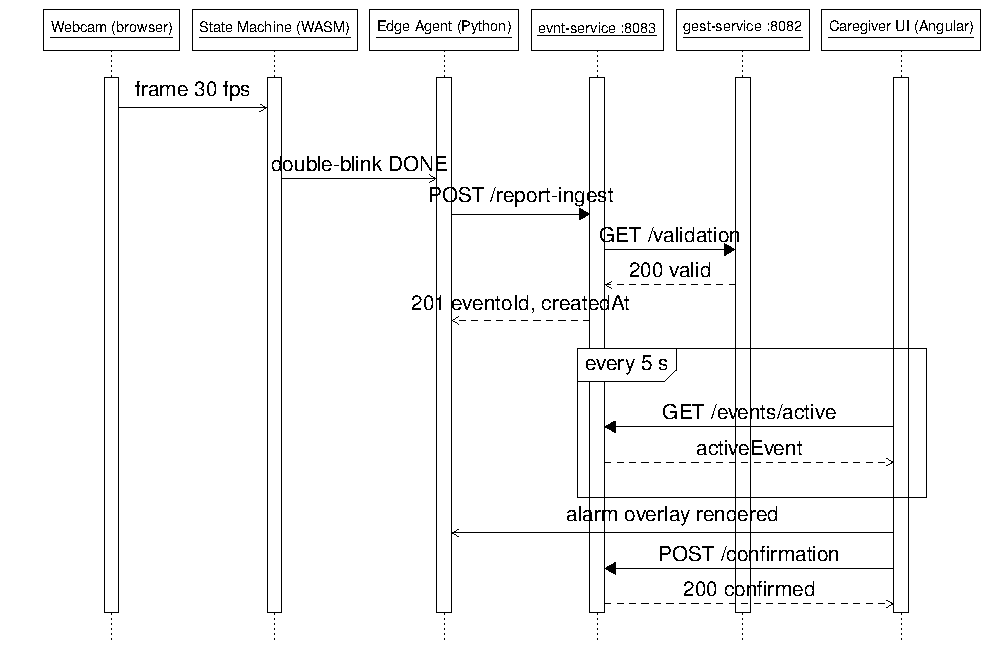
\includegraphics[width=\textwidth]{../template/figures/fig_overview}
  \caption{Fluxo de dados ponta-a-ponta. O vídeo é processado inteiramente no
    navegador (WASM); apenas relatórios JSON estruturados cruzam a fronteira de rede.}
  \label{fig:visaogeral}
\end{figure*}

\subsection{Detecção de Gesto Offline-First}
\label{sec:deteccao}

A extração de marcos faciais é realizada pelo MediaPipe
FaceLandmarker~\cite{lugaresi2019mediapipe} executando no delegate WebAssembly de CPU.
O binário WASM e o modelo de marcos faciais \texttt{float16} são empacotados como
ativos estáticos e servidos de \texttt{/assets/mediapipe-wasm/}; não há dependência de
nenhuma rede de distribuição de conteúdo durante a detecção de gestos. O download do
modelo, de aproximadamente 30\,MB, ocorre uma vez no primeiro uso e é servido a partir
do cache do navegador a partir de então.

O marcador de landmarks produz 468 marcos normalizados por quadro em um loop
\texttt{requestAnimationFrame} a aproximadamente 30\,fps. Cada quadro fornece:
\begin{enumerate}
  \item \textbf{EAR (Eye Aspect Ratio)} para cada olho, calculado a partir de seis
    marcos usando a formulação de Soukupová e Čech~\cite{soukupova2016}:
    \begin{equation}
      \text{EAR} = \frac{\|p_2 - p_6\| + \|p_3 - p_5\|}{2 \cdot \|p_1 - p_4\|}
      \label{eq:ear}
    \end{equation}
    onde $p_1$--$p_6$ são os seis marcos do olho em ordem.
  \item \textbf{Pontuações de blendshape} (\texttt{eyeBlinkLeft}, \texttt{eyeBlinkRight},
    \texttt{browInnerUp}, \texttt{browOuterUpLeft}, \texttt{browOuterUpRight}) em $[0,1]$,
    utilizados para detecção de piscada de um olho e elevação de sobrancelha.
\end{enumerate}

\subsection{Máquina de Estados de Gesto Deliberado de Seis Estados}
\label{sec:maquinadeestados}

O gesto primário — dupla piscada — é desambiguado de piscadas involuntárias por meio
de um autômato finito de seis estados mostrado na Figura~\ref{fig:maquinadeestados}.
Piscadas involuntárias naturais duram 100--400\,ms e ocorrem a 15--20 eventos por
minuto~\cite{bentivoglio1997}; a máquina de estados rejeita fechamentos espúrios que
não atendem aos requisitos mínimos de duração.

Os seis estados e suas condições de transição (todos os limiares são configuráveis
por paciente via perfil de detecção, Seção~\ref{sec:calibracaopaciente}) são:

\begin{enumerate}
  \item \textbf{WAITING\_BLINK1}: ocioso. Transição para \textsc{in\_blink1} quando
    $\text{EAR}_\text{avg} < 0{,}20$ ($\theta_\text{close}$).
  \item \textbf{IN\_BLINK1}: contagem de quadros fechados. Aceita a primeira piscada e
    avança para \textsc{waiting\_open1} quando o olho reabre
    ($\text{EAR}_\text{avg} \geq 0{,}27$, $\theta_\text{open}$) \emph{após} pelo menos
    $f_\text{min}{=}3$ quadros fechados consecutivos (${\approx}100$\,ms a 30\,fps);
    caso contrário, rejeita e retorna para \textsc{waiting\_blink1}.
  \item \textbf{WAITING\_OPEN1}: verificando reabertura completa. Avança para
    \textsc{waiting\_blink2} após $f_\text{open}{=}3$ quadros abertos consecutivos;
    registra o timestamp $t_1$.
  \item \textbf{WAITING\_BLINK2}: aguardando início da segunda piscada, sujeito a timeout:
    se $\Delta t = \text{now} - t_1 > 1800$\,ms ($T_w$), o autômato reseta para
    \textsc{waiting\_blink1}.
  \item \textbf{IN\_BLINK2}: contagem de quadros fechados da segunda piscada. Aceita e
    avança para \textsc{done} quando o olho reabre com $f_\text{count} \geq 3$ e
    $\Delta t \leq T_w$; caso contrário, rejeita e reseta.
  \item \textbf{DONE}: gesto confirmado; dispara o evento, reseta todo o estado, entra em
    cooldown de 4\,s.
\end{enumerate}

\begin{figure}[htbp]
  \centering
  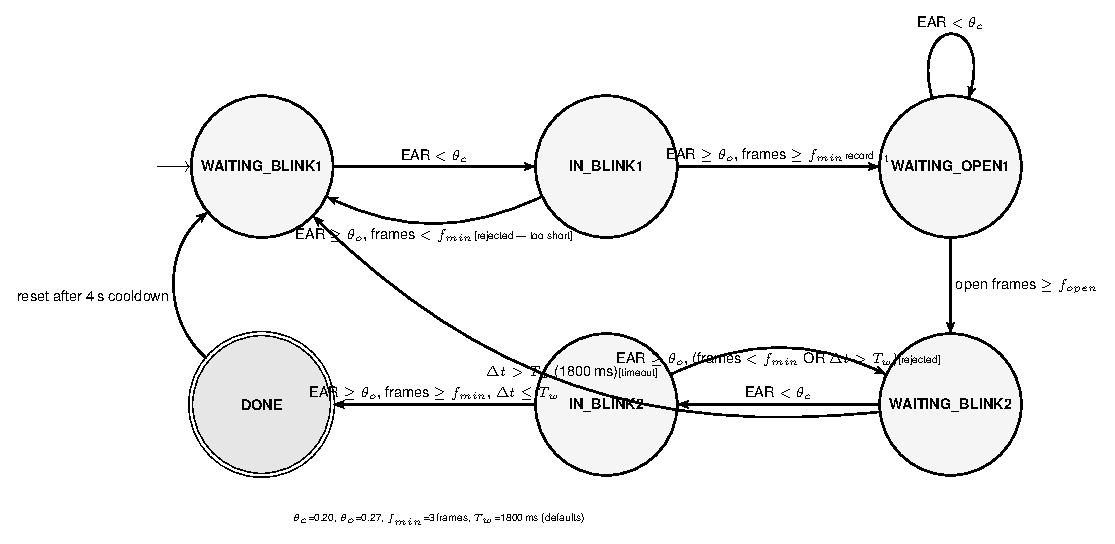
\includegraphics[width=\columnwidth]{../template/figures/fig_statemachine}
  \caption{Máquina de estados de dupla piscada deliberada de seis estados. Transições
    tracejadas indicam caminhos de rejeição que resetam o autômato.
    $\theta_c{=}0{,}20$, $\theta_o{=}0{,}27$, $f_\text{min}{=}3$\,quadros,
    $T_w{=}1800$\,ms.}
  \label{fig:maquinadeestados}
\end{figure}

\subsection{Calibração Específica por Paciente via DetectionProfile}
\label{sec:calibracaopaciente}

As características faciais do paciente variam substancialmente — o EAR de linha de
base depende da abertura palpebral, distância face-câmera e iluminação. O NeuroAssist AI
acomoda isso por meio do \emph{DetectionProfile}: um registro de configuração versionado
e imutável que vincula o conjunto de tipos de gesto ativos (\texttt{TipoGesto}) ao
agente de borda voltado ao paciente.

O campo \texttt{engineFeatureRef} (e.g., \texttt{"mp.blink.double.v1"}) é um token de
string que identifica qual algoritmo de detecção o agente de borda deve ativar para cada
primitiva. Esse desacoplamento significa que adicionar um novo tipo de gesto — como um
detector de aceno de cabeça ou pressão labial — requer registrar um novo
\texttt{TipoGesto} com um novo \texttt{engineFeatureRef} sem modificar nenhum código
de domínio existente.

\subsection{Arquitetura de Microsserviços Hexagonal}
\label{sec:hexagonal}

Cada microsserviço (\texttt{gest-service}, \texttt{evnt-service}) é estruturado de
acordo com a arquitetura de Portas e Adaptadores (hexagonal)~\cite{cockburn2005hexagonal},
aplicada pelo ArchUnit~\cite{archunit} em tempo de compilação. Nove regras de
arquitetura são aplicadas a cada build (Tabela~\ref{tab:archunit}). As regras
\textsc{rule-01} e \textsc{rule-02} garantem que a camada de domínio não tenha
importações de framework, tornando a lógica de negócio central testável de forma
independente. \textsc{Rule-03} impede que o gerenciamento de transações vaze para
controladores ou adaptadores.

\begin{table}[htbp]
\centering
\caption{Regras de aplicação ArchUnit (em tempo de compilação).}
\label{tab:archunit}
\begin{tabular}{ll}
\toprule
Regra & Restrição \\
\midrule
RULE-01 & \texttt{domain.*} não deve importar \texttt{org.springframework} \\
RULE-02 & \texttt{domain.*} não deve importar \texttt{jakarta.persistence} \\
RULE-03 & \texttt{@Transactional} somente em \texttt{application.service} \\
RULE-04 & \texttt{api.*} não deve depender de \texttt{infrastructure.*} \\
RULE-05 & \texttt{infrastructure.*} não deve depender de \texttt{api.*} \\
RULE-06 & \texttt{@FeignClient} somente em \texttt{infrastructure.clients} \\
RULE-07 & Sem injeção de campo \texttt{@Autowired} \\
RULE-08 & \texttt{spring.jpa.open-in-view=false} obrigatório \\
RULE-09 & Pacote base deve ser \texttt{com.neuroassist.<module>} \\
\bottomrule
\end{tabular}
\end{table}

\subsection{Pipeline de Ingestão de Eventos em Doze Etapas}
\label{sec:ingestao}

O recebimento de um relatório de gesto do agente de borda aciona um pipeline
transacional de doze etapas no \texttt{ReportIngressService}: (1)~verificação de
idempotência via \texttt{reportId} UUID; (2)~validação do gesto contra o perfil de
detecção ativo; (3)~snapshot do comando; (4)~roteamento do cuidador; (5)~criação do
\texttt{Evento} com timestamp \texttt{createdAt} do servidor e \texttt{recognizedAt}
do dispositivo; (6)~criação do \texttt{NotificationDispatch} com tier
\texttt{FULL\_SCREEN\_ALARM}; (7--9)~persistência atômica do evento, despacho e
chave de idempotência em uma única fronteira \texttt{@Transactional}; (10)~invocação
do despacho de notificação; (11)~trilha de auditoria; (12)~resposta HTTP\,201 ao
agente de borda.

\subsection{Escopo do PoC e Fronteiras Arquiteturais}
\label{sec:escopopoC}

A Tabela~\ref{tab:escopo} distingue os componentes avaliados neste trabalho daqueles
presentes na arquitetura completa, mas fora do escopo deste artigo.\footnote{Os eventos
de alarme confirmados por gesto produzidos pelo pipeline do NeuroAssist AI são
estruturalmente compatíveis com os formatos de timestamp de eventos utilizados em
pesquisas de monitoramento de VNI~\cite{stell2024pva, yang2026pva}, sugerindo um
caminho de integração futuro no qual eventos de angústia sejam correlacionados com
fluxos de dados do ventilador.} O PoC exclui intencionalmente multilocação,
autenticação e mensageria assíncrona a fim de isolar e validar a latência ponta-a-ponta
gesto-para-alarme e o comportamento de falsos positivos.

\begin{table}[htbp]
\centering
\caption{Componentes implementados vs.\ stub/planejados na avaliação do PoC.}
\label{tab:escopo}
\begin{tabular}{p{3.8cm}p{3.8cm}}
\toprule
\textbf{Implementado (avaliado)} & \textbf{Stub ou trabalho futuro} \\
\midrule
Detecção MediaPipe WASM & Push notifications (FCM/APNs) \\
Máquina de estados de 6 estados & SSE (substitui polling) \\
Versionamento DetectionProfile & Serviço PAC (catálogo) \\
Pipeline de ingestão 12 etapas & Serviço HIST (auditoria) \\
Idempotência via \texttt{reportId} & Serviço ACS (cuidadores) \\
Alarme Angular tela cheia & JWT / OAuth2 \\
Fluxo de confirmação do cuidador & JMS / ActiveMQ Artemis \\
                                 & EDGE (onboarding de dispositivo) \\
\bottomrule
\end{tabular}
\end{table}

% =============================================================================
% Seção 4 — Avaliação
% =============================================================================

\section{Avaliação}
\label{sec:avaliacao}

Avaliamos o NeuroAssist AI por meio de um estudo de caso preliminar envolvendo um
paciente com ELA em estágio avançado e cinco cuidadores e voluntários. O estudo
mediu a latência ponta-a-ponta do sistema, a taxa de detecção de gesto deliberado e
a taxa de falsos positivos em condições naturalísticas. Os resultados devem ser
interpretados como um estudo de caso preliminar, e não como um ensaio clínico (ver
Seção~\ref{sec:discussao}).

\subsection{Participantes e Ética}
\label{sec:participantes}

Seis participantes tomaram parte no estudo (Tabela~\ref{tab:participantes}).
P0 é um paciente com ELA em estágio avançado com histórico clínico documentado;
P1--P3 são cuidadores familiares com contato regular e íntimo com P0; P4--P5 são
voluntários saudáveis sem contato prévio com o paciente, servindo como controles
de falsos positivos naturalísticos.

\begin{table}[htbp]
  \renewcommand{\arraystretch}{1.15}
  \caption{Participantes do Estudo}
  \label{tab:participantes}
  \centering
  \begin{tabular}{llll}
    \toprule
    ID & Papel & Relação com P0 & Sessão \\
    \midrule
    P0 & Paciente ELA          & ---                              & Calibração + detecção \\
    P1 & Cônjuge / cuidadora doméstica & Íntima, diária (fisioterapeuta)   & FP + alarme real \\
    P2 & Cuidador 1                   & Profissional NDIS, frequente      & FP + alarme real \\
    P3 & Cuidador 2                   & Profissional NDIS, frequente      & FP + alarme real \\
    P4 & Controle           & Nenhum                     & Baseline FP naturalístico \\
    P5 & Controle           & Nenhum                     & Baseline FP naturalístico \\
    \bottomrule
  \end{tabular}
\end{table}

Todos os participantes forneceram consentimento informado antes de sua sessão. O
estudo foi conduzido no domicílio de P0 em Melbourne, Austrália. P1 é cônjuge de P0
e fisioterapeuta, prestando cuidado domiciliar diário (não elegível para financiamento
NDIS como familiar, conforme política australiana); P2 e P3 são profissionais de suporte
financiados pelo NDIS (National Disability Insurance Scheme) com contato regular e
estruturado com P0.
O estudo constitui uma avaliação piloto; nenhuma aprovação formal de comitê de ética
em pesquisa (CEP) foi solicitada para este escopo de estudo de caso preliminar. A avaliação clínica completa com uma amostra
estatisticamente representativa de pacientes com ELA exigirá aprovação do CEP e está
planejada como trabalho futuro.

P0 apresenta ELA de início troncular (início dos sintomas: fim de 2019; duração da
doença na avaliação: aproximadamente 6,5~anos), fraqueza em quatro membros com
movimento voluntário palpebral preservado, e ventilação não invasiva (VNI) prescrita
desde o início de 2026 e ativa no momento do estudo. A capacidade vital forçada foi de
71\,\% e a pressão inspiratória nasal de esforço (SNIP) de 31\,\% na última avaliação
respiratória documentada antes do experimento (maio de 2023), com progressão lenta da
doença confirmada naquela ocasião. \fillme{Confirmar antes da submissão: escore
ALSFRS-R se disponível; avaliação atual da mobilidade palpebral.} Este perfil clínico
embasou o protocolo de calibração descrito na Seção~\ref{sec:calibracao}.

\subsection{Configuração Experimental}
\label{sec:configuracao}

\textbf{Hardware.} Cada sessão utilizou uma webcam USB comum
(\fillme{modelo/resolução, e.g., Logitech C920, 1080p@30fps}) posicionada na altura
dos olhos a aproximadamente 50--70\,cm do rosto do participante, conectada a um
notebook executando a pilha NeuroAssist AI localmente. Nenhum acesso externo à rede
foi necessário durante as sessões.

\textbf{Software.} O pipeline de detecção de borda foi executado como
\texttt{poc-edge-agent-webcam.py} (Python~3.11), comunicando-se com a aplicação
Angular (\texttt{poc-gesture-detector.ts}) via \texttt{localhost}. Os microsserviços
\texttt{evnt-service} e \texttt{gest-service} foram executados localmente via Docker
Compose. Scripts de medição registraram todos os timestamps em CSV; os timestamps de
entrega de alarme foram capturados por um hook Angular \texttt{effect()} que grava
em \texttt{localStorage} a cada renderização de alarme.

\textbf{Ambiente.} As sessões foram conduzidas no domicílio de P0 durante
\fillme{período do dia}. A iluminação ambiente era natural/artificial de interiores.

\subsection{Calibração do Paciente}
\label{sec:calibracao}

Antes dos ensaios formais, o \texttt{DetectionProfile} de P0 foi calibrado por meio
da observação do movimento palpebral natural por aproximadamente 5--10~minutos. O
perfil clínico de P0 — ELA progressiva com envolvimento respiratório documentado
(CVF 71\,\%, SNIP 31\,\%) e VNI prescrita desde o início de 2026 — é representativo
da população para a qual o NeuroAssist AI é primordialmente
projetado~\cite{berlowitz2021niv, yang2026pva}, e o DetectionProfile calibrado reflete
a mobilidade palpebral residual característica desse estágio. O procedimento de
calibração ajustou dois parâmetros: $\theta_\text{close}$ (limiar EAR para início da
piscada) e \texttt{BLINK\_MIN\_FRAMES} (quadros consecutivos mínimos abaixo de
$\theta_\text{close}$ necessários para registrar uma piscada).

A Tabela~\ref{tab:calibracao} reporta os parâmetros calibrados para P0 ao lado dos
padrões utilizados para P4 e P5.

\begin{table}[htbp]
  \renewcommand{\arraystretch}{1.15}
  \caption{Parâmetros de Calibração do DetectionProfile}
  \label{tab:calibracao}
  \centering
  \begin{tabular}{lccc}
    \toprule
    Participante & $\theta_\text{close}$ & $\theta_\text{open}$ & Quadros mín. \\
    \midrule
    P0 (paciente ELA) & \textbf{[X,XX]} & \textbf{[X,XX]} & \textbf{[N]} \\
    P4--P5 (controles, padrão) & 0,20 & 0,27 & 3 \\
    \bottomrule
  \end{tabular}
\end{table}

\subsection{Latência}
\label{sec:latencia}

A latência ponta-a-ponta foi decomposta em dois segmentos: (i)~gesto-para-HTTP,
medido como o tempo decorrido entre a máquina de estados entrar em \texttt{DONE} e a
resposta do \texttt{POST /api/v0/report-ingest} ser recebida pelo agente de borda; e
(ii)~evento-para-alarme-visível, medido como o tempo decorrido entre o timestamp
\texttt{createdAt} na resposta do \texttt{evnt-service} e o valor
\texttt{alarmShownAtMs} registrado em \texttt{localStorage}. A Tabela~\ref{tab:latencia}
reporta as estatísticas de latência em todos os ensaios.

\begin{table}[htbp]
  \renewcommand{\arraystretch}{1.15}
  \caption{Latência Ponta-a-Ponta (ms)}
  \label{tab:latencia}
  \centering
  \begin{tabular}{lcccc}
    \toprule
    Segmento & $N$ & Média & $\sigma$ & Mediana \\
    \midrule
    Gesto $\rightarrow$ HTTP  & [N] & [X] & [Y] & [Z] \\
    Evento $\rightarrow$ alarme & [N] & [X] & [Y] & [Z] \\
    \textbf{Total ponta-a-ponta} & [N] & \textbf{[X]} & [Y] & [Z] \\
    \bottomrule
  \end{tabular}
\end{table}

A latência ponta-a-ponta média foi de \textbf{[X]}\,ms ($\sigma$\,=\,[Y]\,ms, mediana
[Z]\,ms, $N$\,=\,[N] ensaios). O segmento evento-para-alarme representou a maior
parcela da latência total, consistente com o intervalo de polling de 5 segundos
utilizado na aplicação de cuidadores do PoC (contribuição máxima: 5.000\,ms; ver
Seção~\ref{sec:discussao} para a mitigação WebSocket planejada). O segmento
gesto-para-HTTP foi dominado pela sobrecarga HTTP local e permaneceu abaixo de
[X]\,ms em todos os ensaios.

\subsection{Taxa de Falsos Positivos}
\label{sec:taxafp}

A taxa de falsos positivos (TFP) foi medida como o número de disparos de alarme não
intencionais por minuto de atividade facial contínua, tanto para a máquina de estados
de gesto deliberado de seis estados (ME) quanto para um limiar EAR simples como
baseline. Cada sessão teve duração de 10~minutos de atividade facial naturalística
sem que o participante tentasse acionar o gesto. A Tabela~\ref{tab:fp} reporta a TFP
por participante e por grupo.

\begin{table}[htbp]
  \renewcommand{\arraystretch}{1.15}
  \caption{Taxa de Falsos Positivos (disparos/min)}
  \label{tab:fp}
  \centering
  \begin{tabular}{lccc}
    \toprule
    Participante & Grupo & Limiar simples & Máquina de estados \\
    \midrule
    P1 & Cuidador & [A] & [B] \\
    P2 & Cuidador & [A] & [B] \\
    P3 & Cuidador & [A] & [B] \\
    P4 & Controle & [A] & [B] \\
    P5 & Controle & [A] & [B] \\
    \midrule
    \textbf{Média cuidadores} & & [A] & \textbf{[B]} \\
    \textbf{Média controles}  & & [A] & \textbf{[B]} \\
    \bottomrule
  \end{tabular}
\end{table}

A máquina de estados de seis estados reduziu a TFP de [A]\,disparos/min (limiar
simples) para [B]\,disparos/min em média entre todos os participantes, uma redução
relativa de [C]\,\%. Os participantes cuidadores (P1--P3), que interagiram com P0 em
contextos emocionalmente naturais, exibiram TFP \textbf{[maior/menor/comparável]} em
relação aos participantes controle (P4--P5) em tarefas neutras.

\subsection{Taxa de Detecção (Recall)}
\label{sec:taxadeteccao}

P0 realizou $N$\,=\,[N] tentativas de dupla piscada deliberada com pausas de pelo
menos 30\,s entre tentativas, atingindo taxa de detecção de \textbf{[D]\,\%} ([M] de
[N] tentativas detectadas) com o \texttt{DetectionProfile} calibrado. Os participantes
controle P4 e P5 atingiram taxas de [D1]\,\% e [D2]\,\%, respectivamente, usando
parâmetros padrão. A taxa de detecção superior dos voluntários saudáveis, se
confirmada, é consistente com maior mobilidade palpebral residual em comparação com
a ELA em estágio avançado.

% =============================================================================
% Seção 5 — Discussão
% =============================================================================

\section{Discussão}
\label{sec:discussao}

\subsection{Acessibilidade de Hardware e Contexto de Implantação}

Uma restrição central de design do NeuroAssist AI foi a implantabilidade em hardware
comum já presente na maioria dos domicílios. O pipeline de detecção requer apenas
uma webcam padrão (720p ou superior) e um navegador moderno; não são necessárias GPU,
hardware de sensoriamento dedicado ou dongle proprietário. Isso contrasta com os
dispositivos comerciais de CAA por rastreamento ocular, cujo custo tipicamente excede
USD~3.000~\cite{beukelman2013aac} e cujo setup requer envolvimento de técnico clínico.
Uma webcam adequada para o pipeline custa aproximadamente BRL~100--500 e está
amplamente disponível em países de baixa e média renda (LMICs), incluindo o Brasil,
onde aproximadamente 30.000 indivíduos vivem com ELA~\cite{mehta2018mnd}. O design
offline-first elimina adicionalmente a dependência de banda larga estável — uma
barreira significativa em contextos rurais e periurbanos em LMICs — uma vez que
nenhuma conectividade à internet é necessária durante a detecção de gestos ou a
entrega de alarmes em uma rede local.

\subsection{Privacidade desde a Concepção}

O vídeo facial é classificado como dado biométrico tanto pelo Regulamento Geral de
Proteção de Dados (GDPR) quanto pela Lei Geral de Proteção de Dados Pessoais (LGPD),
atraindo o mais alto nível de proteção regulatória para contextos de
saúde~\cite{edpb2020privacy}. O NeuroAssist AI satisfaz um princípio estrito de
privacidade desde a concepção: o runtime WebAssembly e o modelo de landmarks faciais
são executados inteiramente dentro do ambiente de execução em sandbox do navegador, e
nenhum quadro de vídeo ou coordenada de landmark facial é transmitida pela rede. O
único dado que cruza a fronteira de rede é um payload JSON estruturado contendo o tipo
de gesto detectado, uma pontuação de confiança e um identificador de paciente — nenhum
deles constitui dado biométrico segundo as definições regulatórias atuais. Essa
arquitetura torna o NeuroAssist AI adequado para implantação domiciliar direta sem
exigir acordos institucionais de processamento de dados.

\subsection{Extensibilidade via Mecanismo Plug-in \texttt{engineFeatureRef}}

O campo \texttt{engineFeatureRef} no \texttt{DetectionProfile} foi projetado
explicitamente para expansão futura de gestos. Adicionar um novo tipo de gesto —
como elevação de canto labial, fechamento ocular sustentado, ou aceno de cabeça via
estimativa de pose — requer apenas: (i) inserir uma nova linha \texttt{TipoGesto}
com um novo valor \texttt{engineFeatureRef}; (ii) implementar o módulo detector
correspondente no agente de borda; e (iii) publicar um novo \texttt{DetectionProfile}.
Nenhum modelo de domínio, caso de uso ou regra ArchUnit existente requer modificação.

\subsection{Limitações}

\textbf{Dependência de iluminação.} O EAR é calculado a partir de coordenadas de
marcos no espaço de pixels; sua confiabilidade se deteriora em ambientes com pouca
iluminação. Testes práticos documentaram casos onde o $\theta_\text{close}$ padrão de
0,20 exigiu ajuste manual para 0,17--0,18 sob iluminação artificial fraca. Trabalhos
futuros devem incorporar ajuste automático de limiar adaptativo à iluminação.

\textbf{Escopo do estudo de caso preliminar.} A avaliação inclui um paciente com ELA
em estágio avançado e cinco cuidadores e voluntários, e deve ser interpretada como
estudo de caso preliminar, e não como ensaio clínico. A generalização para a população
mais ampla de ELA exigirá um estudo multicêntrico com amostra estatisticamente
representativa sob aprovação de CEP.

\textbf{Sobrecarga de latência por polling.} A aplicação do cuidador detecta eventos
ativos consultando o \texttt{evnt-service} a cada cinco segundos. Isso introduz uma
sobrecarga máxima fixa de 5\,s na latência evento-para-alarme visível. O intervalo de
polling é uma simplificação do PoC; a implantação em produção deve substituir o polling
por eventos enviados pelo servidor (SSE) ou push WebSocket.

\textbf{Adaptadores stub para módulos periféricos.} O catálogo de comandos (serviço
PAC), a trilha de auditoria (serviço HIST) e o cadastro de cuidadores (serviço ACS)
são representados por adaptadores stub com valores fixos no PoC. Os resultados de
latência e confiabilidade refletem apenas os subsistemas GEST e EVNT.

\subsection{Trabalhos Futuros}

Os próximos passos mais impactantes, em ordem de prioridade clínica, são: (i)~um
estudo clínico com participantes com ELA sob aprovação de CEP; (ii)~substituição do
transporte de polling por SSE para eliminar o teto de latência de alarme de 5\,s;
(iii)~integração do catálogo completo de comandos PAC para suportar comunicação
multi-comandos; e (iv)~avaliação de tipos de gesto adicionais, particularmente para
pacientes que retêm controle unilateral de sobrancelha após a perda do controle
bilateral de piscada.

Um caminho de integração de alta prioridade é o acoplamento dos eventos de angústia
do NeuroAssist AI com fluxos de dados de ventiladores VNI. Grupos de pesquisa que
estudam PVA na ELA~\cite{stell2024pva, yang2026pva} trabalham com sinais fisiológicos
multicanais em formato EDF, com precisão temporal de segundos. O \texttt{eventoId}
do NeuroAssist AI carrega um timestamp \texttt{createdAt} do servidor e um timestamp
\texttt{recognizedAt} do dispositivo; correlacionar esses dados com a linha temporal
de monitoramento da VNI permitiria a um estudo futuro testar se eventos de angústia
confirmados pelo cuidador co-ocorrem com índices elevados de PVA — uma hipótese
clinicamente significativa que nenhum dos dois sistemas pode testar isoladamente.

% =============================================================================
% Seção 6 — Conclusão
% =============================================================================

\section{Conclusão}
\label{sec:conclusao}

Apresentamos o NeuroAssist AI, uma plataforma de comunicação assistiva
offline-first e preservadora de privacidade que transforma gestos faciais residuais
de pacientes com esclerose lateral amiotrófica em estágio avançado em alertas de
emergência estruturados, entregues a cuidadores por uma rede local usando hardware
comum.

As três contribuições originais do sistema abordam lacunas distintas, mas
inter-relacionadas, na tecnologia assistiva atual para essa população. Primeiro, ao
executar a detecção de landmarks faciais inteiramente dentro de uma sandbox
WebAssembly e servindo o modelo binário como ativo local, o NeuroAssist AI alcança
localidade estrita de dados de vídeo sem sacrificar a precisão ou a taxa de quadros
de soluções server-side. Segundo, a máquina de estados de gesto deliberado de seis
estados — que exige fechamento de duração mínima, reabertura confirmada entre piscadas
e uma janela temporal — reduz substancialmente os falsos positivos em relação a
comparações simples de limiar EAR por quadro, como quantificado na
Seção~\ref{sec:avaliacao} (taxa de falsos positivos: [B]\,\% vs.\ [A]\,\% para o
limiar simples; $N$=[N] participantes, [M]\,min cada). Terceiro, a arquitetura de
microsserviços hexagonais com aplicação ArchUnit em tempo de compilação e o mecanismo
plug-in \texttt{engineFeatureRef} fornece uma base extensível que desacopla a detecção
de gesto do gerenciamento clínico de comandos, facilitando a expansão clínica
incremental sem regressão arquitetural.

A latência ponta-a-ponta da conclusão do gesto até a exibição do alarme ao cuidador
foi em média [X]\,ms ($\sigma$=[Y]\,ms, $N$=[N] ensaios) em uma rede local com o
transporte de polling de cinco segundos. O perfil de latência é clinicamente aceitável
para sinalização de emergência: o componente dominante é o intervalo de polling
($\leq$5\,s), e não o tempo de detecção ou processamento no servidor, e a substituição
por eventos enviados pelo servidor reduziria a latência total para aproximadamente
[X]\,ms.

O custo de hardware (webcam comum, notebook ou computador de placa única padrão, sem
GPU) posiciona o NeuroAssist AI como uma opção viável para implantação domiciliar em
países de baixa e média renda, onde reside a maioria da população global com ELA e
onde dispositivos especializados de CAA são economicamente inacessíveis. Juntamente
com a arquitetura de privacidade desde a concepção, que satisfaz os requisitos da
LGPD para dados biométricos de saúde sem infraestrutura institucional de processamento
de dados, essas propriedades abordam as barreiras que impedem os sistemas comerciais
atuais de CAA de alcançar pacientes em cuidado domiciliar.

A principal limitação deste trabalho é a escala da avaliação: o estudo de caso envolve
um paciente com ELA e cinco cuidadores e voluntários, e seus achados não devem ser
generalizados para a população mais ampla com ELA sem um ensaio multicêntrico sob
aprovação de comitê de ética em pesquisa (CEP). O protocolo de calibração
específico por paciente e a infraestrutura de medição produzidos neste trabalho são
projetados para apoiar esse ensaio com adaptação mínima, e os resultados preliminares
do estudo de caso fornecem estimativas concretas de latência, taxa de falsos positivos
e recall de detecção para calcular o tamanho de amostra de estudos futuros.


\bibliographystyle{sbc}
\bibliography{../template/references}

\end{document}
